\documentclass[a4paper,twoside,titlepage]{article}

\usepackage{a4wide}
\usepackage{hyperref}
\usepackage{graphics}
\usepackage{graphicx}
\usepackage{subfigure}
\usepackage{pifont}
\usepackage{longtable}
\usepackage{listings}
\usepackage{pdflscape}
\usepackage{geometry}
\usepackage{afterpage}
\usepackage{enumitem}
\usepackage{etoolbox}
\lstloadlanguages{XML,XSLT,Java}
\usepackage{verbatim,moreverb}

\newcounter{rownumbers}
\preto\tabular{\setcounter{rownumbers}{0}}
\preto\longtable{\setcounter{rownumbers}{0}}
\newcommand\rownumber{\stepcounter{rownumbers}\arabic{rownumbers}}

\title{Design Document}
\author{Alex Hobson, Hamish O'Keeffe, Lydia Looi, Harry Collard, Alan Wang, Frankie Oprenario}
\date{\today}

\begin{document}
	\maketitle
	\tableofcontents
	
	\newpage
	\renewcommand{\abstractname}{Executive Summary}
	\begin{abstract}
		The client requires our team to produce a Pop-Up Point Of Food Sale system, where the main functionalities include importing existing data files, processing and displaying them in a simple to use GUI where the employees and business owners can interact with and add any new data. Another important feature is the sales screen where employees can take orders, where the corresponding items are removed that the customer orders, automatic checks will be established to make sure that the menu items ingredients will all be in stock, if not an error will be displayed. The main stakeholders are the business owner, employees and developers, these will be the stakeholders that interact with the program most and it is vital that the system is simple enough for the employees to use and also coded in a logical way in order for developers to easily update parts of the system without having to refactor big chunks. The business owner also needs to achieve complex tasks in a simple manner such as deciding what stock to bring to a specific event. 
	\end{abstract}
	
	
\section{Buinsess Information}
\label{sect:buisness}

\subsection{System Context}
\begin{enumerate}
	\item May is a busy food truck owner and wants to keep track of the food that I have in the truck so I know what I need to stock in the truck each morning. Since I am so busy I need the GUI to be easy to use without having to click through lots of menus to do frequent tasks such as entering an order.
	\item I’m a food truck employee and I would like to quickly view the recipes.
	\item I’m a non-native English speaking food truck employee and I would like to enter orders into the program using icons and/or a GUI in my native language.
	\item I’m a customer and would like to view the menu listed from the food truck.
	\item I’m a food truck employee and I would like to know if the food truck has enough stock to make an order before taking payment from a customer.
	\item I’m a food truck employee serving a vegan customer and would like to be able to keep track of how many vegan items are in stock as well as other items for other dietary requirements.
\end{enumerate}

\subsection{Relevant Business Information}
The food truck owner(s) would want to pay for us to develop this PUPOFS as it would save time and money organising and estimating inventory levels, which can lead to the prevention of shortages in stock, or lots of spoilt food.

	
\section{Stakeholders and Requirements}
\label{sect:require}

\subsection{Stakeholders}

\begin{center}
\begin{longtable}{|p{3cm}|p{6.6cm}|p{2cm}|}
\hline \multicolumn{1}{|p{3cm}|}{\textbf{ID (Stakeholder)}} & \multicolumn{1}{|p{6.6cm}|}{\textbf{Description (how they impact the product and/or development process)}} & \multicolumn{1}{|p{2cm}|}{\textbf{Priority}} \\ \hline 
\endfirsthead

\multicolumn{3}{c}%
{{\bfseries \tablename\ \thetable{} -- continued from previous page}} \\
\hline \multicolumn{1}{|p{3cm}|}{\textbf{ID (Stakeholder)}} &
\multicolumn{1}{|p{6.6cm}|}{\textbf{Description (how they impact the product and/or development process)}} &
\multicolumn{1}{|p{2cm}|}{\textbf{Priority}} \\ \hline 
\endhead

\hline
\endlastfoot


Owner & An individual or company that owns the food truck business that intend to serve food to customers and make a profit from the sale. They understand how the food truck should operate and will provide features that can be implemented to make specific processes more efficient & High \\\hline
Manager & An individual who is in charge of the employees and the facilities they work in & High \\\hline
Chef & Person who will prepare and cook food in the kitchen and the food truck based on the menu items established & High \\\hline
Employees & Individuals who work for the food truck business. They may interact with customers to sell food, take orders, process these orders and help prepare food & High \\\hline
Developer & An individual or group that will build and update an application that will be used by the food truck staff and potentially other members. & High \\\hline
Suppliers & Provides products and goods ordered from the business to maintain the stock required for further sales & Low \\\hline
Banks & Handles the finances of the business and also offer other financial benefits & Low \\\hline
General Customer & Potential customers interested in the what the food truck has to offer and possibly buy items & Medium \\\hline
Tourists & Same as a general customer but may speak other languages. Also be able to order and view items but have in a language that is easy for them to understand & Medium \\\hline
Event Organisers & People or companies that can potentially hire a food truck business to cater food for the people attending the organised event & Low \\
\end{longtable}
\end{center}
\newpage
\subsection{Use Case Diagrams}
\begin{figure}[!htb]
	\centering
	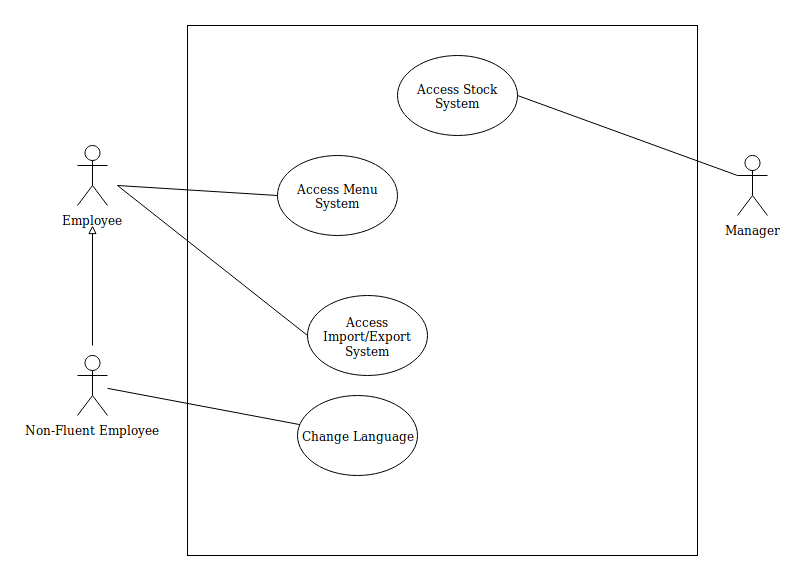
\includegraphics[width=0.7\textwidth]{main_case}
	\caption{Main Use Case}
	\label{fig:maincase}
\end{figure}
\begin{figure}[!htb]
	\centering
	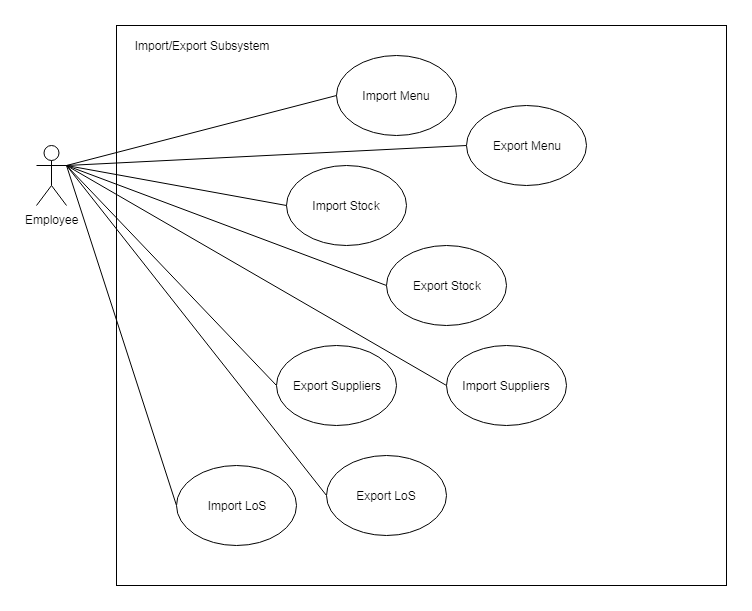
\includegraphics[width=0.7\textwidth]{import_export_case}
	\caption{Import/Export Case}
	\label{fig:iocase}
\end{figure}
\begin{figure}[!htb]
	\centering
	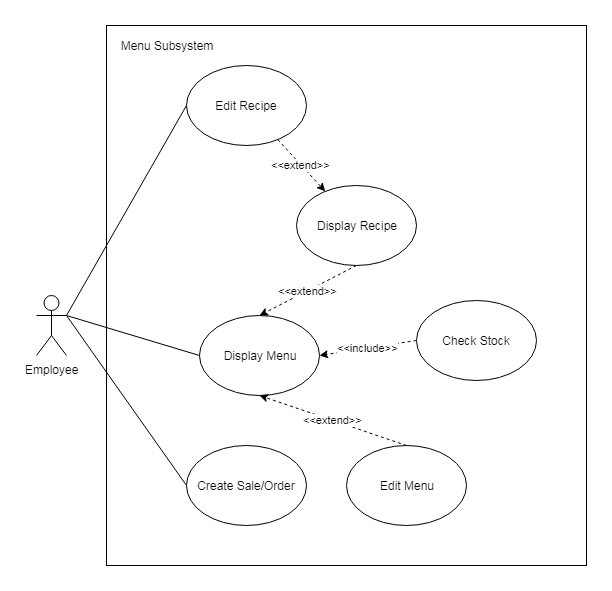
\includegraphics[width=0.7\textwidth]{menu_case}
	\caption{Menu Use Case}
	\label{fig:menucase}
\end{figure}
\begin{figure}[!htb]
	\centering
	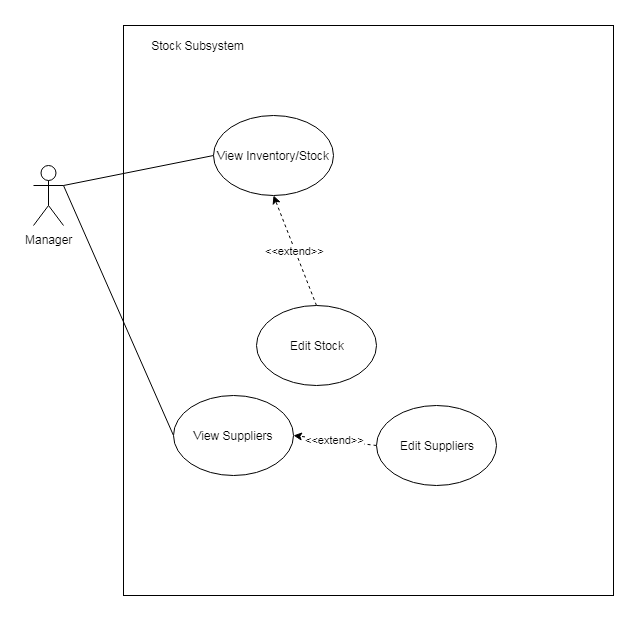
\includegraphics[width=0.7\textwidth]{stock_case}
	\caption{Stock Use Case}
	\label{fig:stockcase}
\end{figure}
\clearpage% Flush earlier floats (otherwise order might not be correct)
\thispagestyle{empty}% empty page style (?)
\begin{landscape}% Landscape page
\subsection{Textual Use Cases}
\begin{longtable}{|p{.05\textwidth}|p{.11\textwidth}|p{.05\textwidth}|p{.1\textwidth}|p{.3\textwidth}|p{.3\textwidth}|p{.1\textwidth}|}
	\hline \multicolumn{1}{|c|}{\textbf{ID}} & \multicolumn{1}{|c|}{\textbf{Name}} & \multicolumn{1}{|c|}{\textbf{Actor}} & \multicolumn{1}{|c|}{\textbf{Preconditions}} & \multicolumn{1}{|c|}{\textbf{Basic Flow}} & \multicolumn{1}{|c|}{\textbf{Exceptional Flow}} & \multicolumn{1}{|c|}{\textbf{Post Conditions}}\\ \hline 
	\endfirsthead
	
	\multicolumn{3}{c}%
	{{\bfseries \tablename\ \thetable{} -- continued from previous page}} \\
	\hline \multicolumn{1}{|c|}{\textbf{ID}} & \multicolumn{1}{|c|}{\textbf{Name}} & \multicolumn{1}{|c|}{\textbf{Actor}} & \multicolumn{1}{|c|}{\textbf{Preconditions}} & \multicolumn{1}{|c|}{\textbf{Basic Flow}} & \multicolumn{1}{|c|}{\textbf{Exceptional Flow}} & \multicolumn{1}{|c|}{\textbf{Post Conditions}}\\ \hline 
	\endhead
	
	\hline
	\endlastfoot
	
	 \rownumber & Display Recipes & Employee & Recipe exists & 
	\begin{enumerate}[wide, labelwidth=!, labelindent=0pt, nosep, topsep=0pt, parsep=0pt]
		\item User clicks on the display recipe button
		\item The screen shows a list of ingredients in each recipe and the required amount of each ingredient
		\item User clicks return button to return to the previous screen
	\end{enumerate} & If no recipes exist:\begin{enumerate}[wide, labelwidth=!, labelindent=0pt, nosep, topsep=0pt, parsep=0pt]
		\item User clicks on the display recipe button
		\item The screen shows an error saying that no recipe exists
		\item User clicks return button to return to the previous screen
	\end{enumerate} & \\\hline
	 \rownumber & Edit Recipes & Employee & Recipe exists & 
\begin{enumerate}[wide, labelwidth=!, labelindent=0pt, nosep, topsep=0pt, parsep=0pt]
	\item User clicks on the edit recipe button
	\item The screen shows a data input screen
	\item The user may change the name, ingredients, and amount of ingredient in recipe
	\item The user clicks a save recipe button
	\item The user is returned to the previous screen
\end{enumerate} & If no recipes exist:\begin{enumerate}[wide, labelwidth=!, labelindent=0pt, nosep, topsep=0pt, parsep=0pt]
	\item User clicks on the edit recipe button
	\item The screen shows a data input screen
	\item The user inputs a recipe name
	\item The user enters the ingredients needed and the required amount
	\item The user clicks a save recipe button
	\item The user is returned to the previous screen
\end{enumerate} & \\\hline
	 \rownumber & Display Recipes & Employee & Recipe exists & 
\begin{enumerate}[wide, labelwidth=!, labelindent=0pt, nosep, topsep=0pt, parsep=0pt]
	\item User clicks on the display recipe button
	\item The screen shows a list of ingredients in each recipe and the required amount of each ingredient
	\item User clicks return button to return to the previous screen
\end{enumerate} & If no recipes exist:\begin{enumerate}[wide, labelwidth=!, labelindent=0pt, nosep, topsep=0pt, parsep=0pt]
	\item User clicks on the display recipe button
	\item The screen shows an error saying that no recipe exists
	\item User clicks return button to return to the previous screen
\end{enumerate} & \\\hline
\end{longtable}
\end{landscape}
\clearpage% Flush page


\end{document}